
\begin{frame}{Research focus}

\begin{itemize}
	\item Direct comparison of two hypothesis.
	\item[i.] \uncover<1->{Phrase scope obligated by the production system, leading to a systematic slowdown for conjoined NPs.}
	\item[ii.] \uncover<1->{Preplanning beyond the first noun is more likely in conjoined NPs but not obligated by the production system.} 


\end{itemize}

\end{frame}


\begin{frame}{Pooled re-analysis}


\begin{itemize}
	\item Stimulus-to-onset latencies
	\item[a.] \textbf{Conjoined NPs:} \textit{The boy and the dog moved above the kite.}
	\item[b.] \textbf{Simple NPs:} \textit{The boy moved above the dog and the kite.}	
\end{itemize}


\begin{itemize}
	\item \textcite{hardy2019age}: 90 ppts; 36 items
	\item \textcite{hardy2020healthy}: 105 ppts; 80 items
	\item \textcite{martin2010planning}: 3$\times$12 ppts; 2$\times$48 and 1$\times$64 items
	\item \textcite{roeser2019advance}: 3$\times$32 ppts; 96 items 
\end{itemize}


\end{frame}


\begin{frame}{Data overview}
	\begin{flushright}
		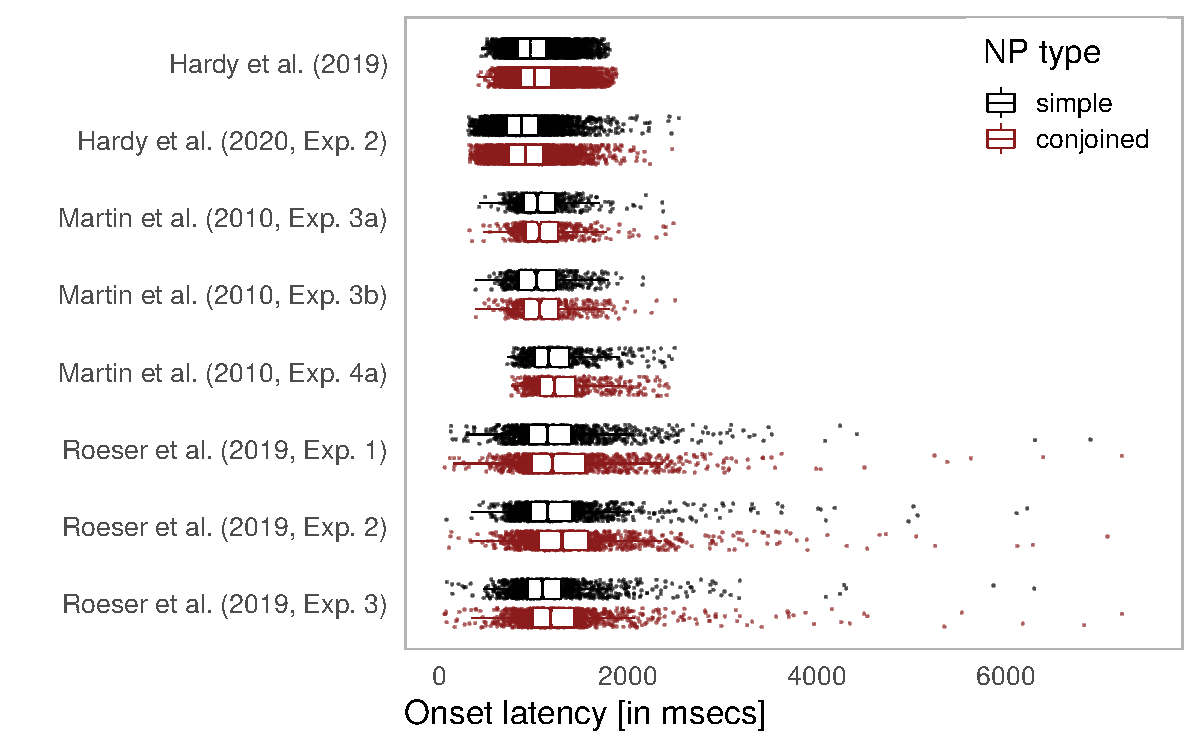
\includegraphics[scale=.5]{metaraw.pdf}
	\end{flushright}
\end{frame}






\begin{frame}[fragile]{Model overview}

\begin{minipage}[t]{.53\textwidth}
\uncover<-2>{
\begin{enumerate}
		\item Null LMM
		\item \textbf{LMM (NP effect)}
		\item LMM (unequal variance)
		\item Null mixture model
		\item \textbf{Mixture model}
\end{enumerate}
\vfill
\begin{itemize}
 	\item Stan code based on \textcite{sorensen2016bayesian} and \textcite{vasishth2017}; also \textcite{vasishth2017feature}.
\end{itemize}

}
\end{minipage}
\hfill
\begin{minipage}[t]{.45\textwidth}
\uncover<2->{
\begin{itemize}
	\item $LogNormal$ distribution with mean $\mu$ and error variance $\sigma_e^2$
	\item Random intercepts 
	\begin{itemize}
		\item participants: $u_i \sim Normal(0, \sigma_u^2)$
		\item items: $w_j \sim Normal(0, \sigma_w^2)$
	\end{itemize}
	\item Weakly informative priors \parencite{mcelreath2016statistical}
\end{itemize}
}
\end{minipage}
	
\end{frame}

\begin{frame}[fragile]{Null model (null hypothesis)}
	
		\begin{equation*}
			\begin{aligned}	
				y_{ij} \sim LogNormal(\mu_{ij}, \sigma_e^2) \\
				\mu_{ij} = \alpha + u_i + w_j\\
			\end{aligned}
		\end{equation*}
\end{frame}


\begin{frame}[fragile]{Meta null model (null hypothesis)}
	
		\begin{equation*}
			\begin{aligned}	
				y_{ijk} \sim LogNormal(\mu_{ijk}, \sigma_{e_k}^2) \\
				\mu_{ijk} = \alpha_k + u_i + w_j\\
				\alpha_k = \alpha_{\mu} + \alpha_{\tau} \cdot \alpha_{\eta_k}\\
			\end{aligned}
		\end{equation*}
		\begin{small}	
			\begin{itemize}
				\item For $k = 1, \dots, K$ where $K$ is the number of studies.
				\item $\alpha_k$ is the latency coefficient for the $k$th study.
				\item $\alpha_{\mu}$ is the pooled latency coefficient.
				\item Non-centred parametrisation for $\alpha_k$ \parencite{gelman2014}.
			\end{itemize}
		\end{small}
\end{frame}


\begin{frame}[fragile]{Meta LMM (standard analysis)}
			
	\begin{equation*}
		\begin{aligned}	
			y_{ijk} \sim LogNormal(\mu_{ijk}, \sigma_{e_k}^2)\\
			\mu_{ijk} = \alpha_k + \beta_k \cdot x_{[0,1]} + u_i + w_j\\
			\alpha_k = \alpha_{\mu} + \alpha_{\tau} \cdot \alpha_{\eta_k}\\
			\beta_k = \beta_{\mu} + \beta_{\tau} \cdot \beta_{\eta_k}\\
		\end{aligned}	
	\end{equation*}		
	\begin{small}	
		\begin{itemize}
			\item $x=0$ for simple NPs; $x=1$ for conjoined NPs.
			\item $\beta_k$ is the latency change for conjoined NPs for the $k$th study.
			\item $\beta_{\mu}$ is the pooled latency change for conjoined NPs.
		\end{itemize}
	\end{small}
	
\end{frame}


\begin{frame}[fragile]{Mixture model (alternative hypothesis)}
	
	\begin{equation*}
		\begin{aligned}
		y_{ij} \sim \theta_{NP} \cdot LogNormal(\mu_{ij} + \delta, \sigma_{e'}^2) + \\
			(1 - \theta_{NP}) \cdot LogNormal(\mu_{ij}, \sigma_{e}^2) \\
			\mu_{ij} = \alpha + u_i + w_j\\
			\text{constraint: }\delta>0\\
			\sigma_{e'}^2 > \sigma_{e}^2 
		\end{aligned}
	\end{equation*}

\uncover<2>{
	\begin{small}
		\begin{itemize}
%			\item $\mu_{ij}$ defined as before.
			\item Probability of long latencies $\theta$ by NP type.
			\item $\mu$ and $\sigma^2$ constant across NP type.
		\end{itemize}
	\end{small}		
}
	
\end{frame}

\begin{frame}[fragile]{Meta mixture model (alternative hypothesis)}

	\begin{equation*}
		\begin{aligned}
		y_{ijk} \sim \theta_{{NP}_k} \cdot LogNormal(\mu_{ijk} + \delta_k, \sigma_{e'_k}^2) + \\
			(1 - \theta_{{NP}_k}) \cdot LogNormal(\mu_{ijk}, \sigma_{e_k}^2) \\
			\mu_{ijk} = \alpha_k + u_i + w_j\\
			\theta_{{NP}_k} = Logit^{-1}(\phi_{{NP}_k})\\
%			\theta_{{NP}} = Logit^{-1}(\phi_{_{\mu_{NP}}})\\		
			\phi_{{NP}_k} \sim Normal(\phi_{\mu_{NP}}, \phi_{\tau}^2)\\
			\delta_k \sim Normal(\delta_{\mu}, \delta_{\tau}^2)\\
			\text{constraint: }\delta_k>0\\
		\end{aligned}
	\end{equation*}
	
	\begin{small}	
		\begin{itemize}
			\item $\alpha_{k}$, $\sigma_{e'_k}^2$, $\sigma_{e_k}^2$ defined as before.
			\item Pooled coefficient for parameters: $\theta_{NP}$, $\delta$
%			\item Inverse-logit for continuous prior on mixing proportion.
		\end{itemize}
	\end{small}
	
\end{frame}


\begin{frame}[fragile]{Meta LMM (unequal variance)}
	\begin{equation*}
		\begin{aligned}
		y_{ijk} \sim
			\begin{dcases*} 
				LogNormal(\mu_{ijk}, \sigma_{e_k}^2), &  if NP$_{ijk}$ = simple\\
				LogNormal(\mu_{ijk} + \beta_k, \sigma_{e'_k}^2) & else if NP$_{ijk}$ = conjoined\\
			\end{dcases*}\\
		\mu_{ijk} = \alpha_k + u_i + w_j\\
		\alpha_k = \alpha_{\mu} + \alpha_{\tau} \cdot \alpha_{\eta_k}\\
		\beta_k = \beta_{\mu} + \beta_{\tau} \cdot \beta_{\eta_k}\\
		\text{constraint: }\sigma_{e_k}^2>0\\
		\sigma_{e'_k}^2 > \sigma_{e_k}^2
		\end{aligned}
	\end{equation*}
	
	
\end{frame}


\begin{comment}
\begin{frame}{Predictions}

\begin{itemize}
	\uncover<-1>	{\item Standard analysis (LMM): Conjoined NPs cause a systematic slowdown in onset latencies, implying that phrase syntax is obligated by the production system.}
	\uncover<2>	{\item Alternative analysis (MoG): Conjoined NPs show a larger probability for longer onset latencies which, however, remain the minority; hence, preplanning syntax is not obligated by the production system.}
\end{itemize}

\end{frame}
\end{comment}



